\documentclass{article}
\usepackage{multicol}
\usepackage[utf8]{inputenc}
\usepackage{float}
\usepackage{graphicx}
\usepackage{hyperref}
\hypersetup{
    colorlinks=true,
    urlcolor=blue,
    }
    
\usepackage{geometry}
\geometry{
    a4paper,
    total={170mm,257mm}
    }

\usepackage{forest}
\definecolor{folderbg}{RGB}{124,166,198}
\definecolor{folderborder}{RGB}{110,144,169}
\def\Size{4pt}
\tikzset{
  folder/.pic={
    \filldraw[draw=folderborder,top color=folderbg!50,bottom color=folderbg]
      (-1.05*\Size,0.2\Size+5pt) rectangle ++(.75*\Size,-0.2\Size-5pt);  
    \filldraw[draw=folderborder,top color=folderbg!50,bottom color=folderbg]
      (-1.15*\Size,-\Size) rectangle (1.15*\Size,\Size);
  }
}

% ------------------------------- FRONT MATTER ------------------------------- %

\title{\textbf{GreenBook}\\~\\
    Third assignment\\
    \small Software Development Process course\\
        University of Milano - Bicocca\\
        A.A. 2021/22\\~\\
        \href{https://gitlab.com/massimino96/2021_assignment3_greenbook/}{Repository Link}}
\author{Authors:\\
    830260 - Binda Paolo - \href{mailto:p.binda@campus.unimib.it}{p.binda@campus.unimib.it}\\
    831075 - D'Apa Massimo - \href{mailto:m.dapa@campus.unimib.it}{m.dapa@campus.unimib.it}\\
    830065 - Fornaro Alessandro - \href{mailto:a.fornaro1@campus.unimib.it}{a.fornaro1@campus.unimib.it}}
\date{}

% ------------------------------- DOC. START ------------------------------- %

\begin{document}
\setlength{\parindent}{0em}
\setlength{\parskip}{1em}

\maketitle
\thispagestyle{empty}

\cleardoublepage
\setcounter{page}{1}

\section*{Introduction}

Due to the outbreak of the recent COVID-19 pandemic, we found it useful to develop a web-app that would facilitate the traceability of possible infections for managers of clubs and restaurants. In fact, COVID virus can easily spread within a restaurant in the presence of many people in the same closed environment.

GreenBook is a Spring web-app that allows to manage reservations in a restaurant, with a particular focus on the traceability of possible COVID infections.

\section*{ER Model Design}
\begin{figure}[H]
    \centering
    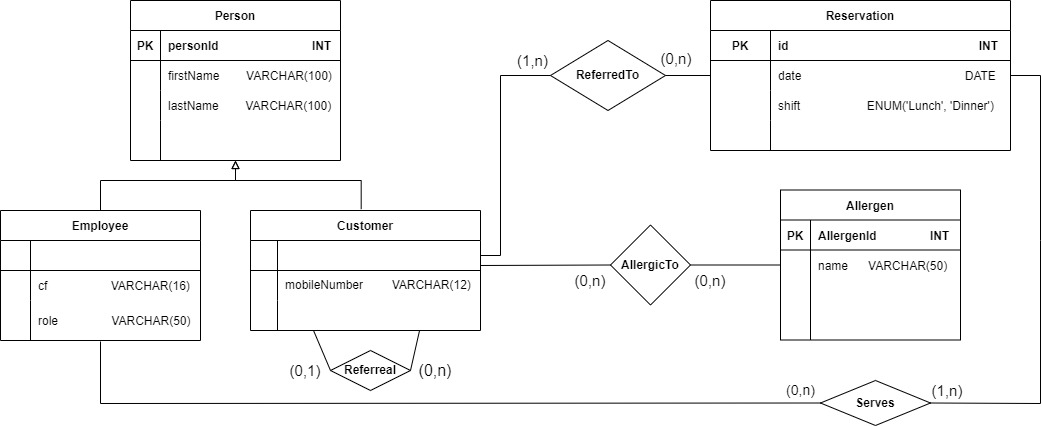
\includegraphics[width=\textwidth]{ER}
    \caption{ER Model}
    \label{fig:ermodel}
\end{figure}

In the phase of ER Design, we made the following assumptions:
\begin{itemize}
  \item A user cannot recommend himself
  \item We trace also employees which are selected for each reservation, as they could be infected and, in such cases, we need to be able to track them too
\end{itemize}

\section*{Web-app Functionalities}
The restaurant staff can mainly perform four types of operations:
\begin{itemize}
    \item Manage reservations: it is the core functionality of the web-app which allows staff to record bookings requested by customers (see below for further details).
    \item Manage employees: this functionality allows the restaurant staff to manage the actual employees, that is, add, edit or remove an employee.
    \item Manage customers: the staff can also see the list of all the customers registered in the restaurant database, insert new customers, edit them and delete them.
    \item Manage allergens: although it is not a core feature for the application, every customer has his special needs and this web-app permits to record possible allergies of each customer.
\end{itemize}

\subsection*{Manage reservations}
[Placeholder: subsection needed?]

\clearpage
\section*{Source code elements}
\begin{multicols*}{2}
{\footnotesize\noindent
    \begin{forest}
      for tree={
        font=\ttfamily,
        grow'=0,
        child anchor=west,
        parent anchor=south,
        anchor=west,
        calign=first,
        inner xsep=7pt,
        edge path={
          \noexpand\path [draw, \forestoption{edge}]
          (!u.south west) +(7.5pt,0) |- (.child anchor) pic {folder} \forestoption{edge label};
        },
        file/.style={edge path={\noexpand\path [draw, \forestoption{edge}]
          (!u.south west) +(7.5pt,0) |- (.child anchor) \forestoption{edge label};},
          inner xsep=2pt,font=\ttfamily
                     },
        before typesetting nodes={
          if n=1
            {insert before={[,phantom]}}
            {}
        },
        fit=band,
        before computing xy={l=15pt},
      }
    [GreenBook
    [src/main/java/it.unimib.bdf.GreenBook
      [controllers
        [AllergenController]
        [CustomerController]
        [EmployeeController]
        [NewReservationController]
        [ReservationController]
        [SearchReservationController]
      ]
      [models
        [Allergen]
        [Customer]
        [Plugin]
        [Employee]
        [Person]
        [Reservation]
        [ReservationListContainer]
      ]
      [repositories
        [AllergenRepository]
        [CustomerRepository]
        [EmployeeRepository]
        [ReservationRepository]
      ]
      [services
        [AllergenService]
        [CustomerService]
        [EmployeeService]
        [ReservationService]
      ]
      [GreenBookApplication.java, file]
    ]
    [resources/WEB-INF
      [jsp
        [allergen]
        [customer]
        [employee]
        [reservation]
        [error.jsp, file]
      ]
      [index.html, file]
    ]
    ]
    \end{forest}
}\columnbreak

The code we have developed is mainly divided into two categories: the one necessary for the implementation of the back-end, written in Java, and the one for the front-end, written in JSP (and of course HTML, CSS and JS). The former is located in the \textit{java/src} directory, while the latter is located in \textit{resources/WEB-INF}.

\subsection*{Front-end}
The front-end was created by defining a page for each functionality offered by the application. Each of these is in fact dedicated to carrying out CRUD functions on specific entities (allergen/customer/employee). The pages in the reservation directory allow the insertion and search of reservations, thus also implementing operations that require the involvement of multiple database entities.

\subsection*{Back-end}
The back-end is dedicated to the management of GET and POST requests made by by the user through the forms presented in the View.

Each entity implements three kinds of classes:
\begin{itemize}
    \item Repository: persistence layer (mechanism for storage, retrieval, search, update and delete operations)
    \item Service: service layer (business logic)
    \item Controller: presentation layer (manage GET and POST requests)
\end{itemize}
\end{multicols*}

\end{document}
